\chapter{Preliminaries}
\label{chapter:prelemenaries}

\section{Data Series And Similarity Search}

A \textbf{data series (DS)} of size (or dimensionality) \( n \) is a sequence 
of \( n \) pairs, where each pair consists of a real value and its corresponding 
dimension.
% 
The \textbf{Piecewise Aggregate Approximation (PAA)}~\cite{DBLP:journals/kais/KeoghCPM01} 
provides a compact representation of a data series by dividing the x-axis into 
\( w \) equal segments. Each segment is then represented by the \textbf{mean value} 
of the corresponding points, as shown by the black horizontal lines in 
Figure~\ref{fig:PAA}. 
% 
\bl{
The PAA representation of a data series \( T = (t_1, t_2, \dots, t_n) \) is computed by 
dividing it into \( w \) segments, each containing \( \frac{n}{w} \) data points. The 
\( i \)-th PAA coefficient \( \overline{t}_i \) is given by:  

\begin{equation}
\overline{t}_i = \frac{w}{n} \sum_{j=\frac{n}{w} (i-1) + 1}^{\frac{n}{w} i} t_j
\label{eq:paa-transformation}
\end{equation}
% 
where the summation aggregates all values in the segment, and the factor \( \frac{w}{n} \) 
ensures proper scaling.  
}
% 
To compute the \textbf{iSAX summary}~\cite{shieh2008sax}, the y-axis is partitioned 
into \( c \) discrete regions, where \( c \) represents the \textbf{cardinality} 
of the representation.
%
Each region is assigned a unique bit pattern, and instead of storing the raw PAA values, 
iSAX encodes each segment using the bit representation of the region it falls into. 
This forms a \textbf{symbolic representation} of the series, 
such as the word \( 10_2 00_2 11_2 \) in Figure~\ref{fig:iSAXSummary} 
(where subscripts indicate the number of bits used per segment).
% 
The number of bits used per region can vary, enabling the construction of a 
\textbf{hierarchical tree index}, known as an \textbf{iSAX-based tree index}, as 
illustrated in Figure~\ref{fig:iSAXTree}.
The index is a \textbf{leaf-oriented tree}, where each leaf stores up to \( M \) keys.
% 
During insertion, if the target leaf \( \ell \) has available space, the new key 
is simply added. However, if \( \ell \) is full, it undergoes a \textbf{split operation},
where it is replaced by a small subtree consisting of an \textbf{internal node} and two 
new leaves, which inherit  the keys from \( \ell \). If one of the newly created leaves
remains empty, the splitting process continues recursively.
For further details on iSAX-based indexes, refer to~\cite{isaxfamily}.


\begin{figure}[htbp]
    \centering
    \begin{subfigure}[b]{0.35\textwidth}
        \centering
        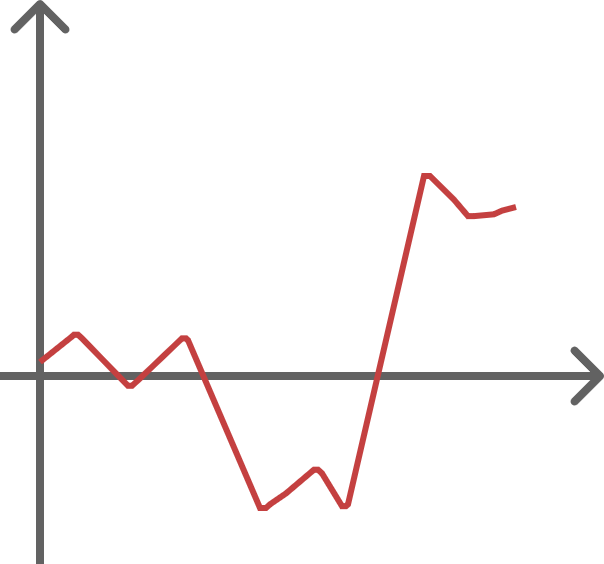
\includegraphics[width=\textwidth]{figures/prelem/timeseries.png}
        \caption{Data Series}
        \label{fig:dataseries}
    \end{subfigure}
    \hfill
    \begin{subfigure}[b]{0.35\textwidth}
        \centering
        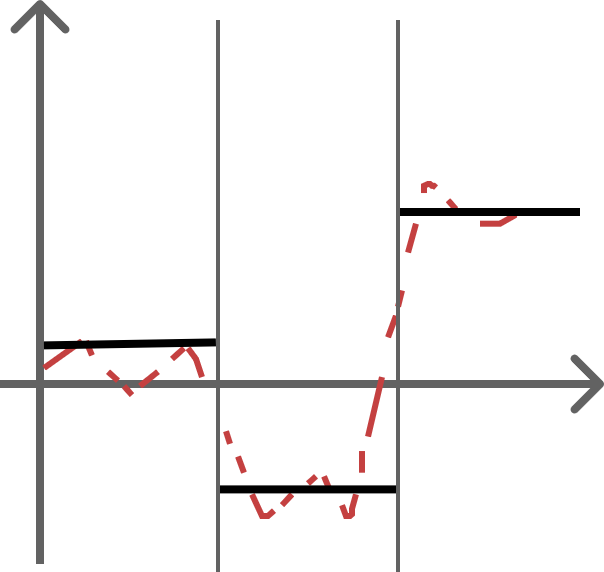
\includegraphics[width=\textwidth]{figures/prelem/PAA.png}
        \caption{PAA Summary}
        \label{fig:PAA}
    \end{subfigure}
    \hfill
    \begin{subfigure}[b]{0.45\textwidth}
        \centering
        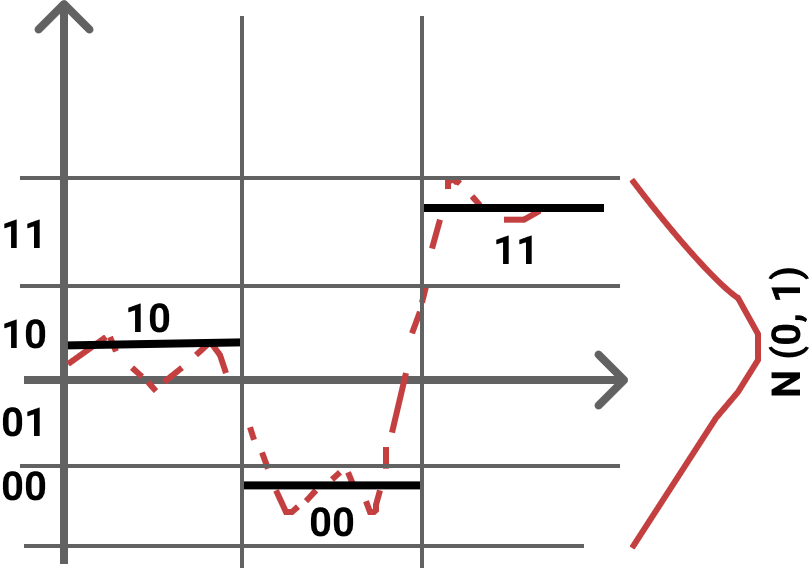
\includegraphics[width=\textwidth]{figures/prelem/isax.png}
        \caption{iSAX Summary}
        \label{fig:iSAXSummary}
    \end{subfigure}
    \hfill
    \begin{subfigure}[b]{0.8\textwidth}
        \centering
        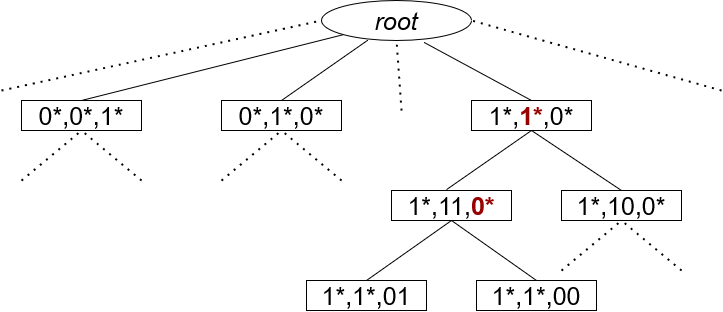
\includegraphics[width=\textwidth]{figures/prelem/isaxTreeCustom.png}
        \caption{iSAX Tree}
        \label{fig:iSAXTree}
    \end{subfigure}
    
    \caption{From data series to iSAX index}
    \label{fig:from_ds_to_iSAX}
\end{figure}

\noindent{\bf Similarity Search}  
We focus on \textit{exact similarity search} (also known as exact \textit{1-NN}),  
which retrieves the data series from a collection that is most similar to a given 
query series. Similarity is typically measured using \textbf{Euclidean Distance (ED)},
but our techniques are general enough to support other widely used 
\textit{similarity measures}, such as Dynamic Time Warping (DTW)~\cite{rakthanmanon2012searching}.  
% 
The \textbf{Euclidean distance} between two time series  
\( T = \{t_1, ... , t_n\} \) and \( T' = \{t'_1, ... , t'_n\} \)  
is defined as:  
\begin{equation}
ED(T, T') = \sqrt{\sum_{i=1}^{n} (t_i - t'_i)^2}
\label{eq:Euclidean-distance}
\end{equation} 
% 
We refer to the distance between the \textit{iSAX summaries} of two data series  
as the \textbf{lower-bound distance}. \bl{If we transform the original subsequences into PAA
representations, $\overline{T}$ and $\overline{T'}$, using Eq.~\ref{eq:paa-transformation}
(according to~\cite{Lin2007SAX}),
we can then obtain a lower bounding approximation of the Euclidean distance
between the original subsequences by:

\begin{equation}
DR(\overline{T}, \overline{T'}) \equiv \sqrt{\frac{n}{w}} \sqrt{\sum_{i=1}^{w} (\overline{t}_{i} - \overline{t'}_{i})^2}
\label{eq:lower-bound-distance}
\end{equation}
}
% 
The calculation of this distance guarantees the \textbf{pruning property}:  
the lower-bound distance between two data series is always less than or equal to  
their Euclidean distance, which we refer to as the \textbf{real distance}.  
% 
This property enables efficient pruning of candidates during query processing:  
a data series can be \textbf{pruned} if its lower-bound distance to the query series
\( Q \) is greater than the real distance of any other data series in the collection 
from \( Q \).

\noindent
{\bf Leaf-Oriented Trees.}  
In a \textit{leaf-oriented tree}, all data are stored in the leaves, with each leaf
capable of holding up to \( M \) keys.  
% 
During an insertion, if the target leaf \( \ell \) has available space,  
the new key is simply added to \( \ell \).  
However, if \( \ell \) is full, it undergoes a \textbf{split}: it is replaced 
by a subtree consisting of an internal node and two new leaves.  
The keys from \( \ell \) are then redistributed between the new leaves based on
their values.  
% 
If one of the newly created leaves remains empty after redistribution,  
the splitting process is repeated until both leaves contain keys.  

\section{iSAX-Based Indexing}

Concurrent iSAX-based indexes~\cite{peng2018paris,parisplus,peng2020messi,  
PFP21-I,PFP21-II} operate in two main phases:  
the \textit{tree index construction phase} and the \textit{query answering phase},  
each utilizing distinct data structures. 

\noindent\textbf{Tree Index Construction.} During this phase a set of \textit{worker threads}  
processes a collection of input data series (i.e., \textit{raw data}).  
Each series is summarized using an iSAX representation and inserted into a 
\textit{tree index} as a pair of an iSAX summary and a pointer to the corresponding 
data series.  
% 
The process is divided into two main stages:
\begin{itemize} [noitemsep, topsep=3pt, partopsep=0pt, parsep=0pt]
    \item \textbf{Buffers Creation:} iSAX summary pairs are first stored in array-based  
    \textit{summarization buffers}.  
    \item \textbf{Tree Population:} Worker threads traverse these buffers and insert 
    their entries into the tree index.  
\end{itemize}  
Data series with similar iSAX representations are placed in the same buffer and later  
within the same subtree of the index tree.  
This approach ensures \textbf{high parallelism}, \textbf{good locality}, and  
\textbf{low synchronization overhead} during index construction.

\noindent\textbf{Query Answering.}  
Given a query data series \( Q \), the system follows these steps
to find the data series with the smallest distance to \( Q \) :  
\vspace{-5pt} % Reduce space before the enumerate list
\begin{enumerate}[noitemsep, topsep=1pt, partopsep=0pt, parsep=0pt]
    \item The iSAX summary of \( Q \) is computed and used to traverse the index tree,  
    leading to a leaf \( \ell \).  
    \item The \textit{real distance} between \( Q \) and each data series in \( \ell \) is computed.  
    \item The smallest distance found so far is stored in the \textbf{Best-So-Far (BSF)} variable,  
    serving as an initial approximate answer.  
\end{enumerate}  
% 
Then query answering proceeds by exexuting the following two stages
namely the \textit{Prunning Stage} and the \textit{Refinement Stage}:

\noindent\textbf{Pruning Stage:} In this stage, a set of \textit{query answering threads}
traverse the tree. If the \textit{lower bound distance} from a node to $Q$
exceeds the Best So Far (BSF) value, the node is \textit{pruned} and excluded from
further processing. This pruning ensures that no pruned data series can contribute
to the final answer.

\noindent\textbf{Refinement Stage:} During refinement, the non pruned data series 
are the candidate series and are stored in one or more \textit{priority queues}~\cite{parisplus,PFP21-I,PFP21-II}.
Multiple threads process these candidate data series, calculating their exact
distances to Q. The BSF is updated whenever a smaller distance is encountered.

At the end of this phase, the final answer is contained in BSF.  
\textit{Barriers} synchronize threads at the end of each stage, ensuring correctness,  
while \textit{locks} handle concurrent access to shared data structures.  
Figures~\ref{fig:example} and~\ref{fig:example2} summarize the indexing process.  

\begin{figure}[H]
    \centering
    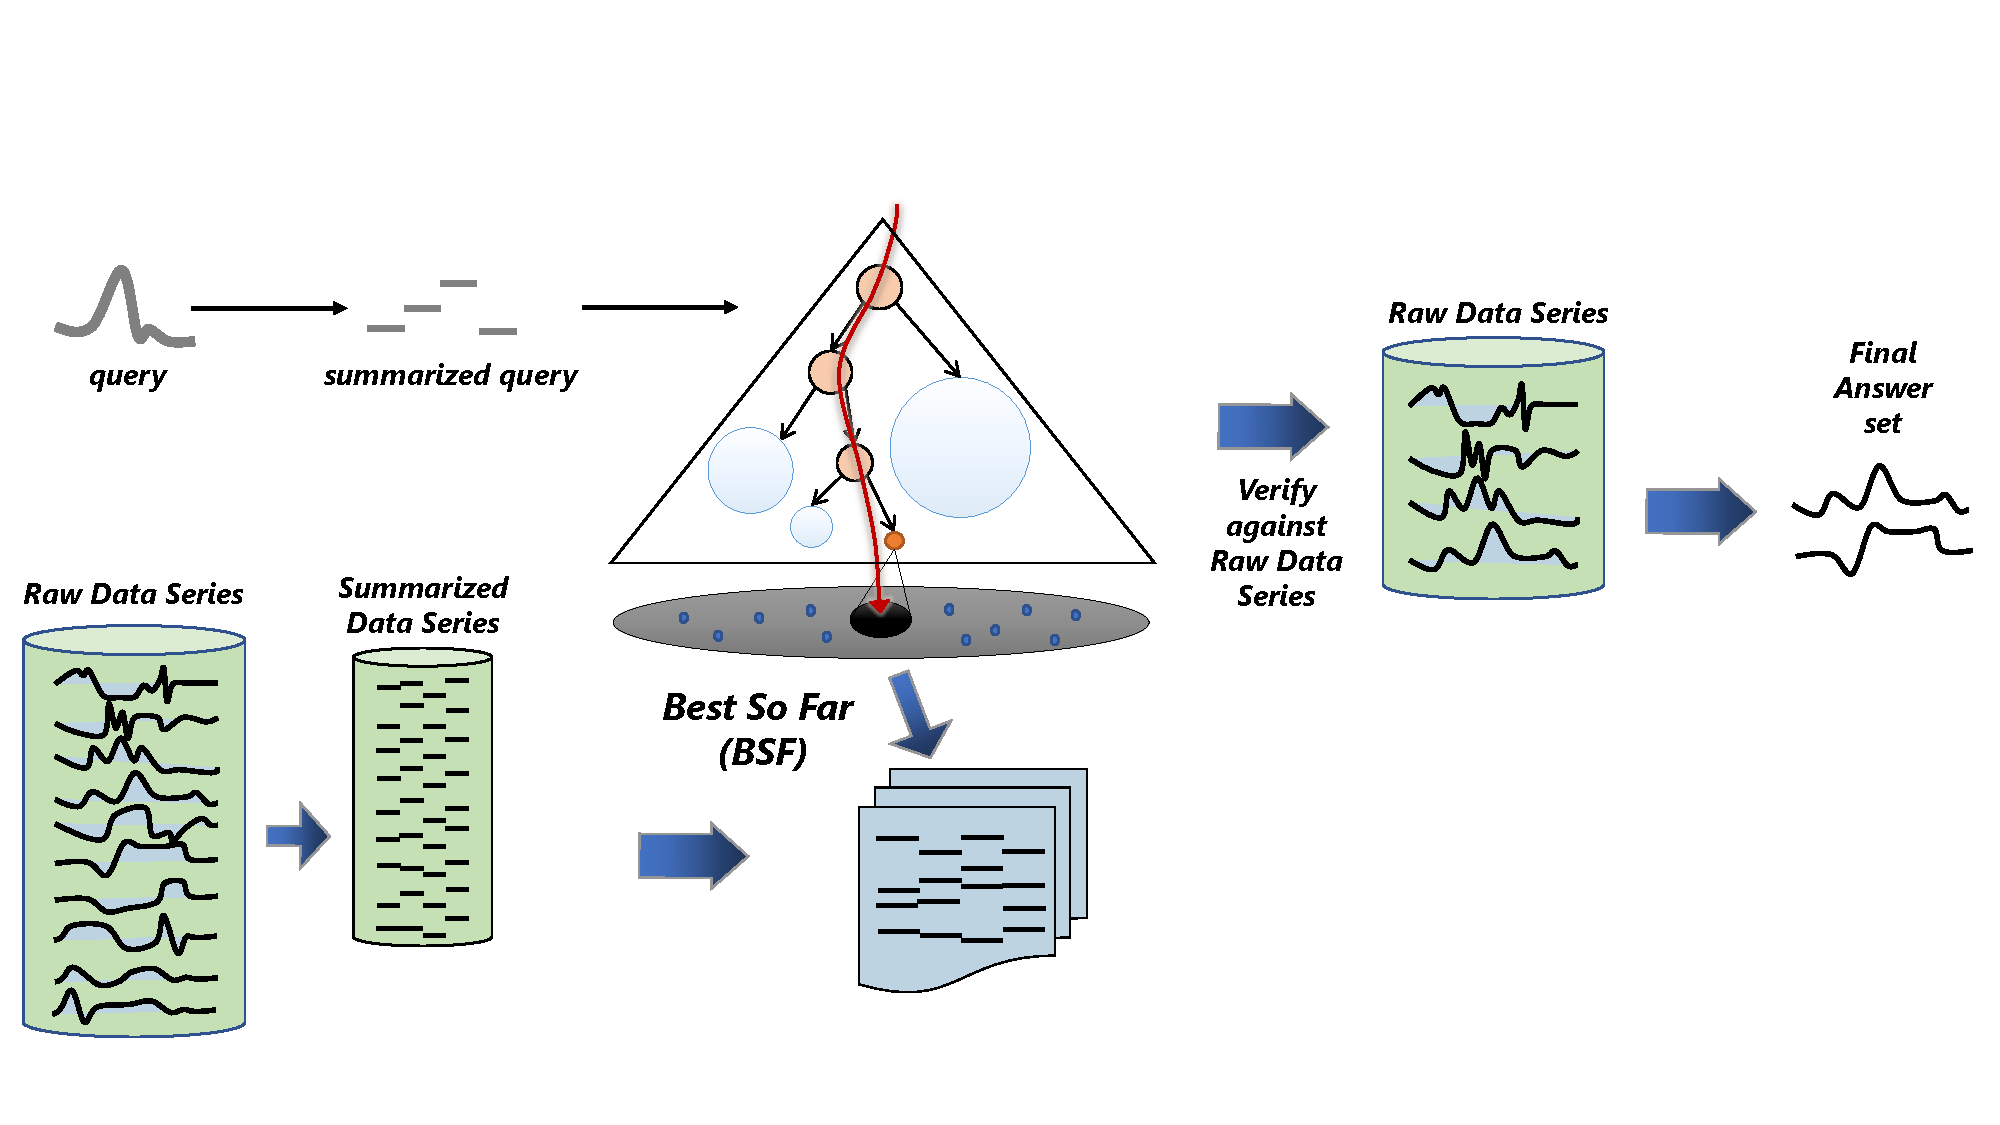
\includegraphics[width=0.85\textwidth]{figures/prelem/iSAX-index.pdf}
    \caption{Similarity search with the use of a data series index.}
    \label{fig:example}
    \vspace{-0.5cm} % Reduces space after the figure
\end{figure}

\begin{figure}[H]
    \centering
    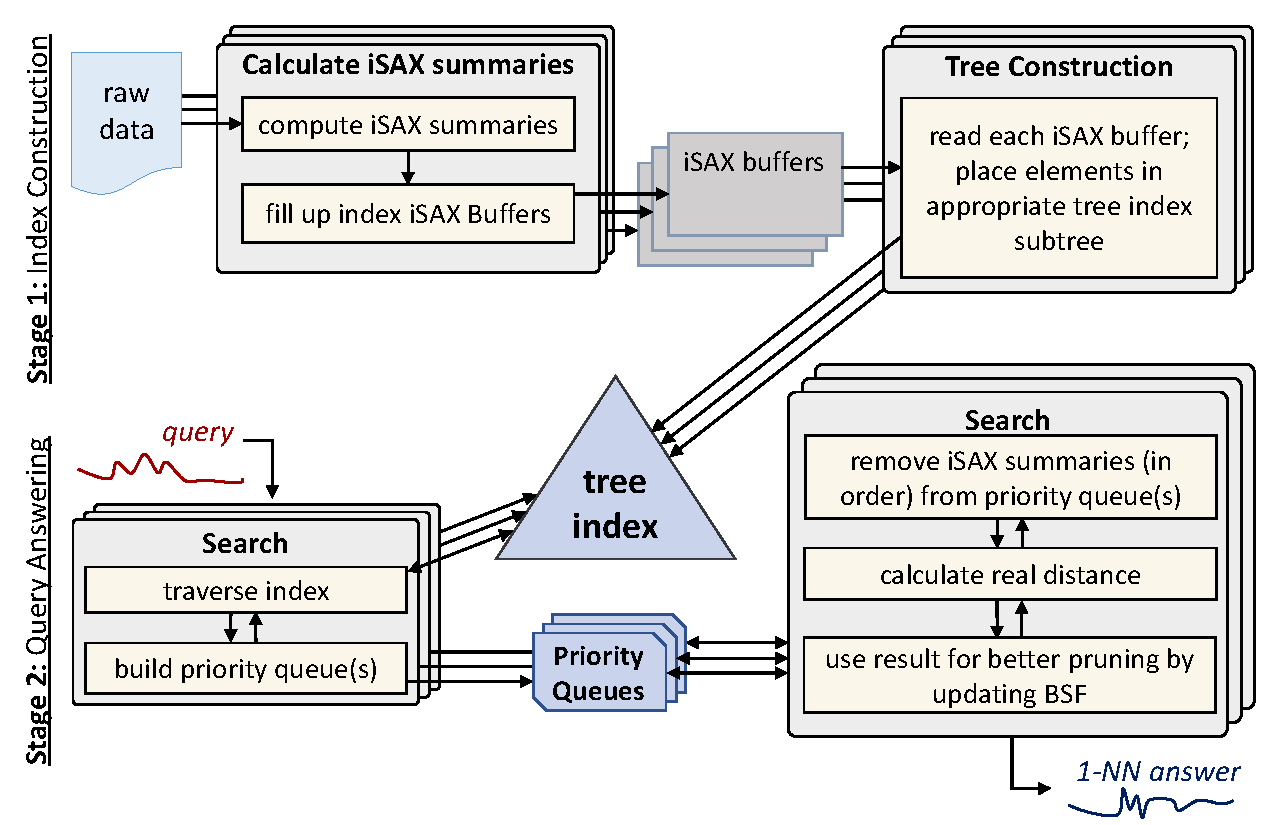
\includegraphics[width=0.8\textwidth]{figures/prelem/flowchart2.pdf}
    \caption{Index building and query answering flowchart for the MESSI data series index.}
    \label{fig:example2}
    \vspace{-0.5cm} % Reduces space after the figure
\end{figure}


\noindent{\bf MESSI as an example.} 
MESSI~\cite{peng2020messi} is a state-of-the-art, in-memory iSAX-based index.
It uses an array, referred to as \textit{RawData}, to store the raw data. During the 
{\em buffers creation stage}, this array is split into a number of fixed-size chunks 
containing consecutive raw data series. A Worker thread repeatedly {\em acquires} and
processes a chunk, storing the calculated iSAX summaries in the appropriate 
summarization buffers. Threads determine which chunks to work on using a \FAI\ object.
Each thread is allocated its own space in each summary buffer to avoid collisions when
adding elements, ensuring thread safety. This process continues until all data series in
\textit{RawData} have been processed.
% 
During the {\em tree population stage}, worker threads again use \FAI\ to {\em acquire}
iSAX buffers to work on. Each subtree of the index tree is a binary leaf-oriented tree
with fat leaves.
% 
In the {\em query answering phase}, a query answering worker repeatedly {\em acquires}
a subtree (using \FAI) and {\em traverses} it by calculating the {\em lower-bound
distance} between the query series \( Q \) and the iSAX summary of each node
encountered. If the lower-bound distance of a leaf is smaller than the Best So Far (BSF)
distance, the leaf is inserted into a {\em priority queue}, with the distance
used as the priority. The algorithm uses a set of {\em priority queues} and threads 
insert elements into these queues in a round-robin fashion.
Since a priority queue may be concurrently accessed by multiple threads, 
MESSI employs a coarse-grain {\em lock} for each queue for synchronization.
% 
During the {\em refinement phase}, each query answering thread \( t \) is assigned a 
priority queue \( \mathit{PQ} \) to process. It repeatedly removes the leaf with the
minimum priority from \( \mathit{PQ} \) and compares its iSAX summary to the BSF.
If the leaf's summary is smaller, the real distances between the data series stored
in the leaf and the query series are computed. Otherwise, the leaf and all remaining
nodes in the queue are pruned. Since multiple threads may process a priority queue
concurrently, it is protected by a coarse-grain lock. Once processing of a priority
queue is complete, thread \( t \) moves on to the next priority queue in a round-robin
manner.
% 
{\em Barriers} are used among threads at the end of each stage and before the start of 
the next to ensure correct synchronization and maintain the integrity of the process.

\section{System And Dynamic Data}
\noindent{\bf System:}
We consider a shared-memory system with \( N \) threads that execute {\em concurrently
and asynchronously} while communicating by accessing shared objects. A shared object
\( O \) can be atomically read or written. Additionally, the operation \FAI(O, v)
atomically reads the current value of \( O \), adds the value \( v \) to it, and
returns the value that was read. The operation \CAS($O, u, v$) reads the value of
\( O \), and if it is equal to \( u \), it changes it to \( v \) and returns
\textit{True}; otherwise, \( O \) remains unchanged and \textit{False} is returned.
% 
Threads may experience delays (e.g., due to page faults, power consumption issues,
or overheating~\cite{inteloverheating}), or they may fail by crashing (e.g., due to
software errors). An algorithm is said to be {\em blocking} if a thread must wait for
actions to be performed by other threads in order to make progress. {\em Lock-freedom}
guarantees that some thread makes progress at each point in time, thus 
the system as a whole continues to make progress independently of the speed of threads
or their failures. Lock-Free algorithms do not utilize locks, MESSI is not lock-free;
it is blocking.


 
\noindent{\bf Dynamic Data:} To simulate dynamicity in data we assume that all data is initially stored in memory, but
only a small subset is used to create the initial index. The rest of the data are organized into batches.
After the initial index is built, new data arrives dynamically in batches, with the batch size
configurable by the user. To simulate real-time data ingestion, we introduce a delay interval
between consecutive batches. This delay, which can be defined by the user,
begins as soon as a batch arrives. By appropriately tuning with the delay we simulate different
dynamicity patterns in data. 
% 
The behavior of the system depends on the interplay between batch size and delay interval.
If the delay is determined to be long enough, index workers (i.e., threads responsible for building the index)
may fully integrate each batch into the index before the next batch arrives, remaining idle for
the rest of the time. Conversely, if the delay is determined to be short or the batch size is large, new batches
may arrive before previous ones have been fully processed.
% 
While index workers are responsible for inserting new data, query workers (i.e., threads
responsible for answering queries) simultaneously access this data to perform
exact similarity search. Ensuring correctness in such a system requires a robust mechanism to
manage concurrent updates and queries. To achieve this, we employ two models inspired by different
domains of computer science: a \textit{timestamp-based model} and a \textit{consistency model based
on linearizability}.  

\subsection{Timestamp-Based Ordering And Linearizability}  

A well-known approach for handling dynamic data is the use of timestamps to enforce ordering 
constraints. This method is widely used in database systems to ensure that data is processed
in a meaningful manner~\cite{babcock2002}. Notable systems employing timestamp-based mechanisms
include Apache Kafka and Google Spanner~\cite{kafka2021,spanner2013}.  
% 
In our approach, timestamps are implicitly generated using the system's clock. Specifically,
every batch is assigned a timestamp corresponding to the time when the processing of the batch
starts. This timestamp plays a crucial role in  how queries behave. Specifficaly,   

\begin{itemize} [noitemsep, topsep=3pt, partopsep=0pt, parsep=0pt]
    \item Queries must see all data that previous queries have seen.  
    \item If a query has a later timestamp than an ongoing batch, it must wait for that batch to
     finish processing before continuing.  
\end{itemize}  
% 
By enforcing this ordering, we ensure that queries always operate on a consistent view of the data.
Our approach is inspired by the principles outlined in \textit{Models and Issues in Data Stream
Systems}~\cite{babcock2002}, which guided the design and implementation of timestamps in our dynamic system.  

The second approach we employ is inspired by \textit{linearizability}
\cite{herlihyWingLinearizability}, a key concept in concurrent
and distributed systems. Linearizability provides a strong consistency guarantee by ensuring
that all operations appear to execute atomically in a single, consistent order.  

Formally, a system execution is \textbf{linearizable} if:  
\begin{itemize}  [noitemsep, topsep=3pt, partopsep=0pt, parsep=0pt]
    \item For each completed operation p, to insert a
    linearization point *p somewhere between p's
    invocation and response in a.
    \item To select a subset F of the incomplete operations,
    and for each operation r in F:
    to select a response, and
    to insert a linearization point *r somewhere after r's invocation in a.
    \item These operations and responses should be selected and these 
    linearization points should be inserted, so
    that, in the sequential execution constructed by
    serially executing each operation at the point that
    its linearization point has been inserted, the
    response of each operation is the same as that in a
\end{itemize} 
% 
By leveraging the principles of linearizability, we ensure that concurrent updates and queries
interact correctly, preserving system correctness while maintaining high concurrency. 
% 
The Timestamp and Linearizability models complement each other by addressing different
aspects of correctness in a dynamic, concurrent system, reflecting the principles of two
distinct domains: the database world and the concurrent computing world.
The timestamp model requires queries to wait for ongoing batches to finish before starting
their processing. This ensures that any batch arriving before or concurrently with the query
will be considered. This approach is generally preferred in the field of databases, as it
respects the temporal sequence of batch arrivals and processing.
On the other hand, linearizability offers more concurrency, as there is no waiting time.
While data arrives, the algorithm is responsible for handling it, ensuring that the execution
remains linearizable. This allows for concurrent operation throughout the entire process of
insertions. 
